Figure~\ref{architecture} shows the framework designed to support our method. This framework offers specific tools that help the design and aggregation of tasks, which are essential activities to put our proposed method in practice.

%\begin{figure*}[ht!]
%	\centerline{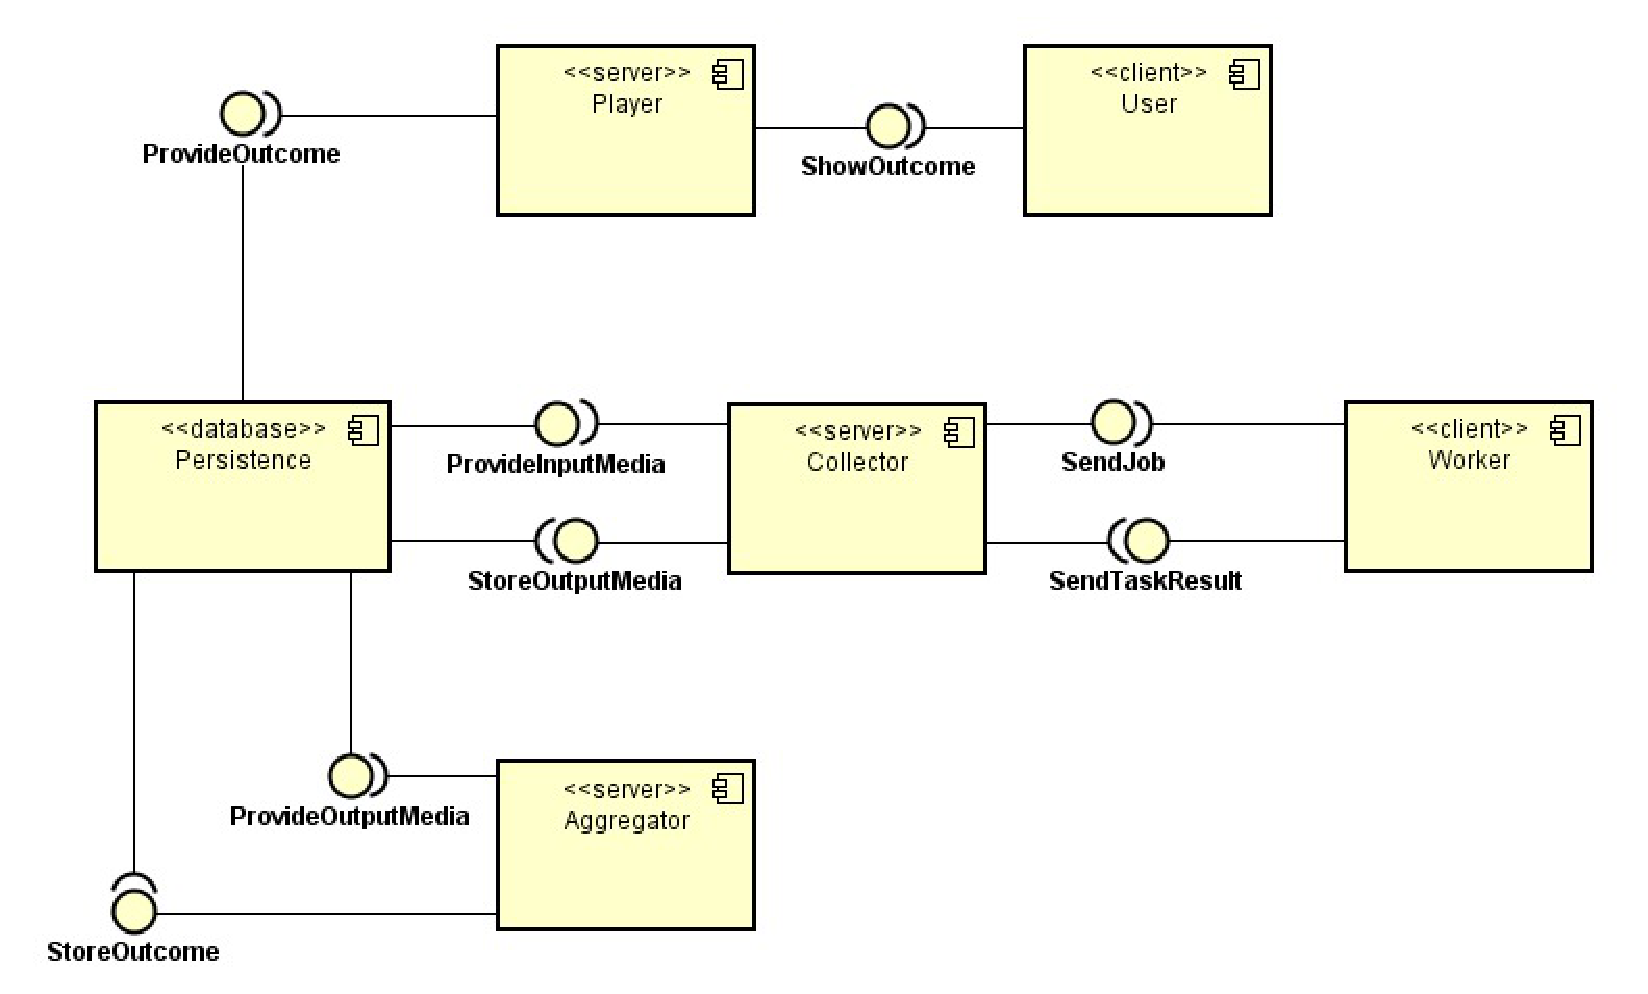
\includegraphics[scale=0.5] {figure/system}}
%	\caption{Framework Architecture}
%	\label{architecture}
%\end{figure*}

\subsection{Database}
%The database module contains the persistence component that is the point of communication between the modules of the structure. In this way, the modules can be decoupled, increasing the flexibility of the system and the possibilities of integration with external environments in a service-oriented architecture. 
%The communication interfaces between the persistence component and the others can be seen in Figure~\ref{persistence}.

%\begin{figure}[h!]
%	\centerline{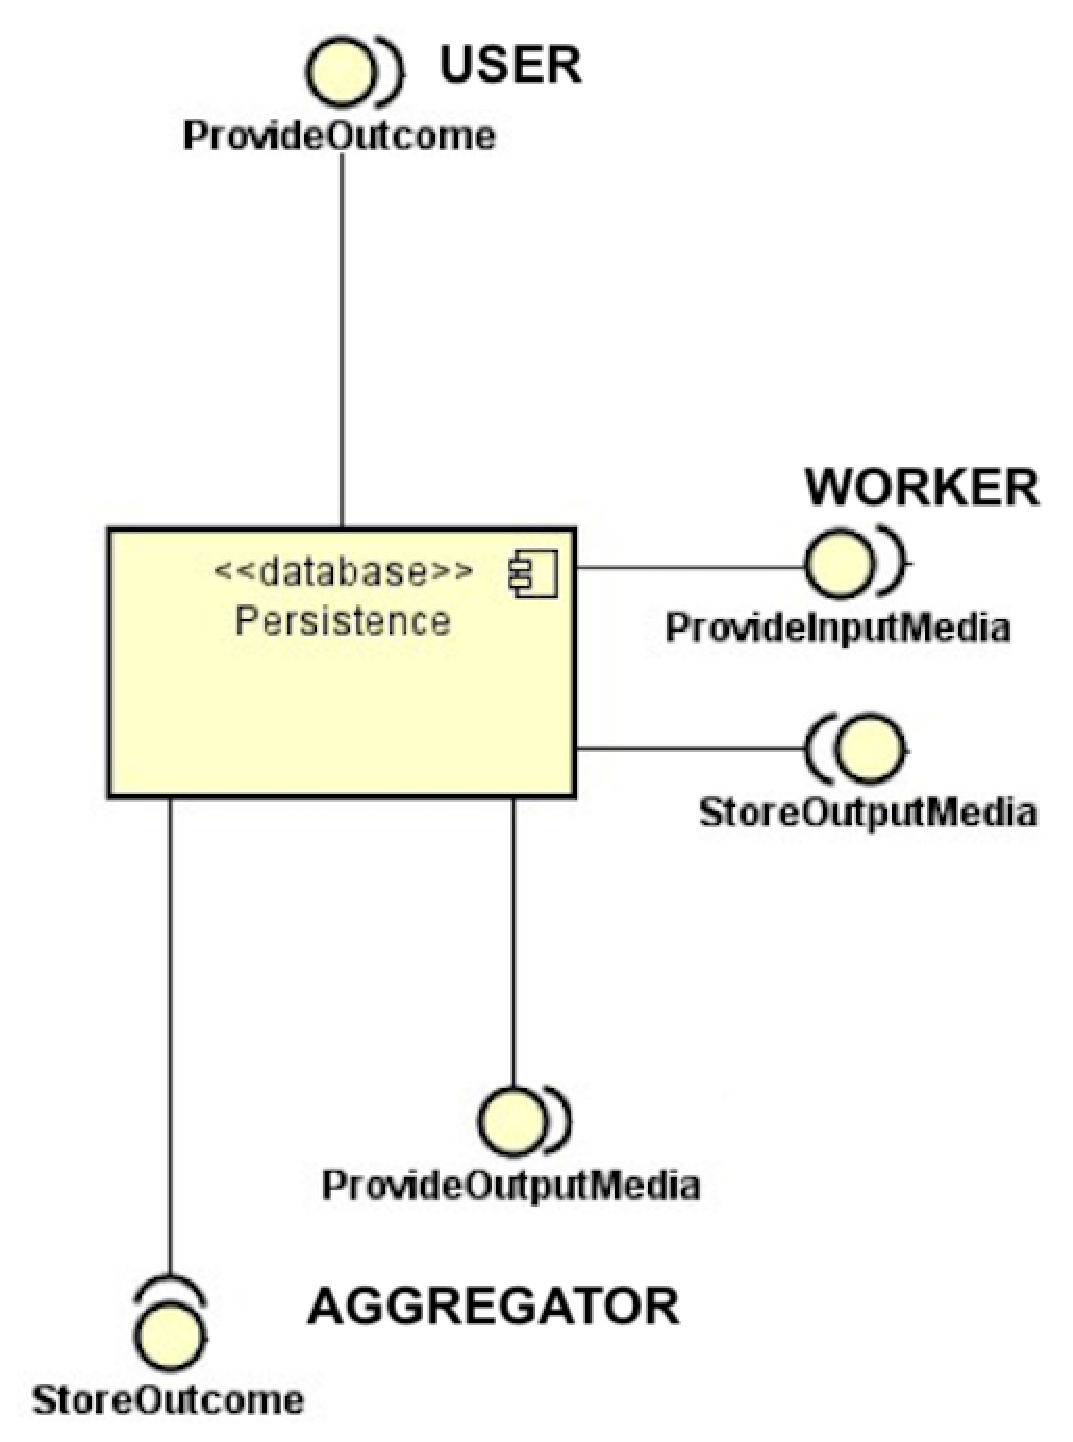
\includegraphics[scale=0.25] {figure/persistence}}
%	\caption{Persistence component}
%	\label{persistence}
%\end{figure}


The persistence component sends to the server module the information required to render in the client both, the job requests to workers and the content needed to present the result to the users. Once the persistence component communicates with its own database.
%, there is no need for the crowdsourcing platform, if used, to have access to the dataset.

Likewise, contributions provided by workers are sent directly from the collector to the persistence component, so that they are stored directly in the database without having to go through the external crowdsourcing environment in no time

The aggregation component also communicates directly with persistence. The aggregator requests each run the collected contributions to a task and, after the aggregation process, sends the result to be stored from the database to be used as input to the next task, again maintaining data privacy because it does not need to be stored in any external environment.

\subsection{Server}
The server module is responsible for distributing the jobs, managing contributions, and controlling the active task in order to execute the process workflow. This module is composed of three components: Collector, Aggregator, and Player. 

\begin{itemize}
\item \textbf{Collector: } The collector feeds an annotation tool with the information about the item to be annotated, so it renders the job's interface used by the worker to perform the task. Completely, this component is also responsible for gathering the information provided by the worker in the execution of the task and sends them to the persistence so that they are stored.

\item \textbf{Aggregator: }The aggregator verifies, filters, groups, and processes the collected annotations of the crowd according to the rules defined for each task. In this update version, the aggregation process can be fully automatic, supervised or manual. Manual aggregation is useful when is desired to evaluate each contribution as in authoring tasks. Supervise aggregation can be a good option when is possible to apply automatic methods but is required human verification of the result. Automatic aggregation is the default choice, this class of methods includes grouping, comparing, counting, calculating and other operations.

\item \textbf{Player: } The player component works in a  similar way to the collector, although it renders the content to users and its communication with the persistence is unidirectional. It feeds the client player tool with the metadata, the extra content, and the original video. Thus, the player tool on the client can play the enriched video synchronously.
\end{itemize}


\subsection{Client}
The client module manages the communication interfaces with workers and users. The approach used is to use templates that are fed with the descriptive data of the visualization to be generated.

In this way, it is possible to keep the entire control part on the server, accessible through the collector and player components, and therefore templates can be stored anywhere if it is accessible on the internet. This allows contributions to be collected from crowdsourcing platforms and web pages published on different hosts. In fact, this strategy allows to collect entries from different sources at the same time.

Both the container collection view and the final content view display work in a similar fashion. According to the desired visualization, a model is selected and the server module is queried to obtain the necessary data to render the desired interface. 

%This process is illustrated in Figure~\ref{rendering}.



%\begin{figure}[h!]
%	\centerline{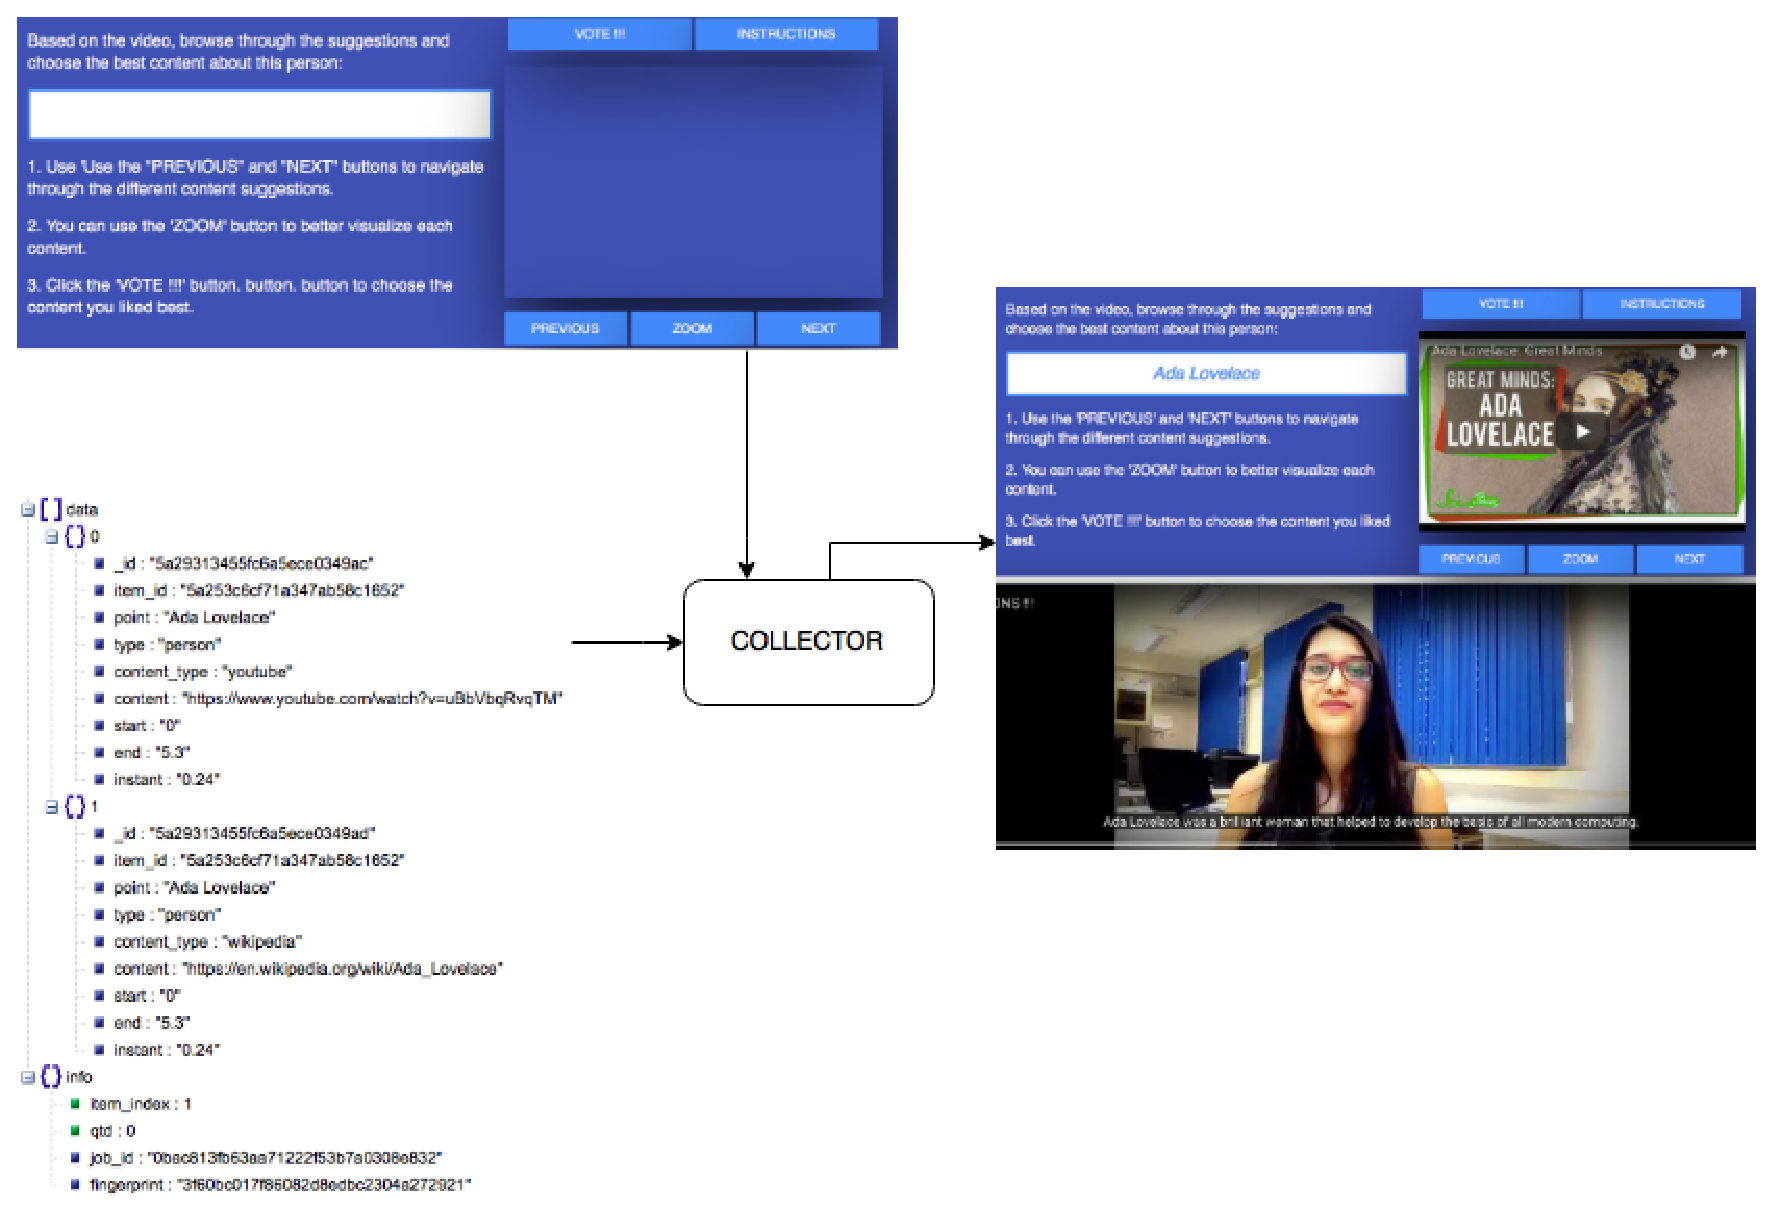
\includegraphics[scale=0.28] {figure/rendering}}
%	\caption{Job rendering}
%	\label{rendering}
%\end{figure}


The interaction between the system modules through the interfaces are described as follow:
\begin{itemize}
\item \textbf{Provide Media Input:} To generate each job to be sent to a worker, the Collector receives an entry from the Persistence component.

\item \textbf{Send Job:} The Collector sends a job to a Worker who sees the task through the Client and executes it.

\item \textbf{Send Job Result:} The Client sends to the Collector the annotation made by the Worker for the job received.

\item \textbf{Store Media Input:} The Collector sends the collected contribution to the Persistence that stores it in the Database.

\item \textbf{Provide Output Media:} The Persistence send to the Aggregator all the collected contributions for a task.

\item \textbf{Store Outcome:} The Aggregator stores the resulting entries from the aggregation process in the Input collection so that they are supplied as input to the next task.

\item \textbf{Provide Outcome:} The Aggregator sends the outcome to Persistence to store it.

\item \textbf{Show Outcome:} The Player displays to a User the outcome generated by the cascading microtasks process.

\end{itemize}

The next section describes how we used this framework to apply our method in a video enrichment case study.















